\documentclass[a4paper, 12pt]{article}
\title{}
\usepackage{geometry}
\usepackage{float}
\usepackage{subfigure}
\usepackage[justification=centering]{caption}
\usepackage{enumerate}
\usepackage{multirow}
\usepackage{listings}
\lstset{
    escapechar=`,
    language=C++,
    numbers=left,
    tabsize=2,
    prebreak=\raisebox{0ex}[0ex][0ex]{\ensuremath{\hookleftarrow}},
    frame=single,
    breaklines=true,
}
\usepackage{graphicx}
\graphicspath{ {./} }
\usepackage{nameref}
\usepackage{amsmath}
\usepackage{amssymb}
\usepackage{amsfonts}
\usepackage[linesnumbered,ruled]{algorithm2e}
\usepackage{tikz}
\usetikzlibrary{calc,patterns,decorations.pathmorphing,decorations.markings,positioning,automata}
\usepackage{pgfplots}
\usepackage{pgfplotstable}
\usepackage{makecell}

\begin{document}
%\maketitle

\section*{Part II: Implementation} \label{sec:intro}
The purpose of this exercise was to use the Finite Element Method (FEM) 
to approximate, and study, the solution to the problem presented in 
Eq. \ref{eq:StrongForm}.

\begin{align}
-(p(x)u'(x))' + q(x) u(x) &= f(x)  \label{eq:StrongForm} \\
u(0) = \alpha , u(1) = \beta  &
\end{align}

\noindent
This equation was solved on the domain $x\in[0,1]$. 
The analytical solution was assumed to exist uniquely.
The variables in Eq. \ref{eq:StrongForm} are as denoted below in Eq. \ref{eq:GivenConds}.

\begin{align} \label{eq:GivenConds}
u(x)\in & C^2 [0,1]  & \\
f,q \in & C^0 [0,1] \quad & q \geq 0\\
p   \in & C^1 [0,1] \quad &p > 0
\end{align}

\noindent
The problem domain of one unit in one dimension was divided into a nonuniform but structured mesh.
The rule for determining element size is shown in Eq. \ref{eq:ElemSize}.

\[
  h_{j} = \begin{cases} 
    0.9 \Delta x \quad \text{ for odd j}  \label{eq:ElemSize} \\
    1.1 \Delta x \quad \text{ for even j}
  \end{cases}
\]

\noindent
The $\Delta x$ referred to in Eq. \ref{eq:ElemSize} is the average size of any given element. 
Specifically, it is calculated by use of Eq. \ref{eq:DeltaX}.

\begin{equation} \label{eq:DeltaX}
\Delta x = \frac{1}{N+1}
\end{equation}

\noindent
Here, $N$ is the number of degrees of freedom; $N+1$ is the number of elements.
Tests were conducted for $N=10, 20, 40, 80, 160, 320$. 
These six mesh size tests were conducted for six different cases which are described in 
Table \ref{tab:Cases}.

\begin{center}
\begin{tabular}{ |c|c|c|c|c|c|}
  \hline
  Case Number & $\alpha$ & $\beta$ & $p$ & $q$ & $u$ \\
  \hline
  1           &   0      &  0      &  3  &  2  &  $u=x(x-1)(sin(5x)+3e^x)$ \\
  \hline
  2           &   0      &  0      &  $p=1+x$  &  0  &  $u=x(x-1)(sin(5x)+3e^x)$ \\
  \hline
  3           &   4      &  4      &  3  &  2  &  $u=4$ \\
  \hline
  4           &   -2     &  -1     &  3  &  2  &  $u=x-2$ \\
  \hline
  5           &   -3     &  -2     &  3  &  2  &  $u=x^2-3$ \\
  \hline
\end{tabular} \label{tab:Cases}
\end{center}

\noindent
A computer code was written to evaluate the posed problems. 
The results follow this section and the code itself is appended to this report.
Plots of the error for $N = 10, 20, 40$ with respect to location are
presented in Figures \ref{fig:Error1} and Figure \ref{fig:Error2}.
Tabulated data, in the form of error norms and convergence order 
are presented in Tables \ref{tab:C1} through \ref{tab:C5}.

\begin{figure}[H]
  \centering
  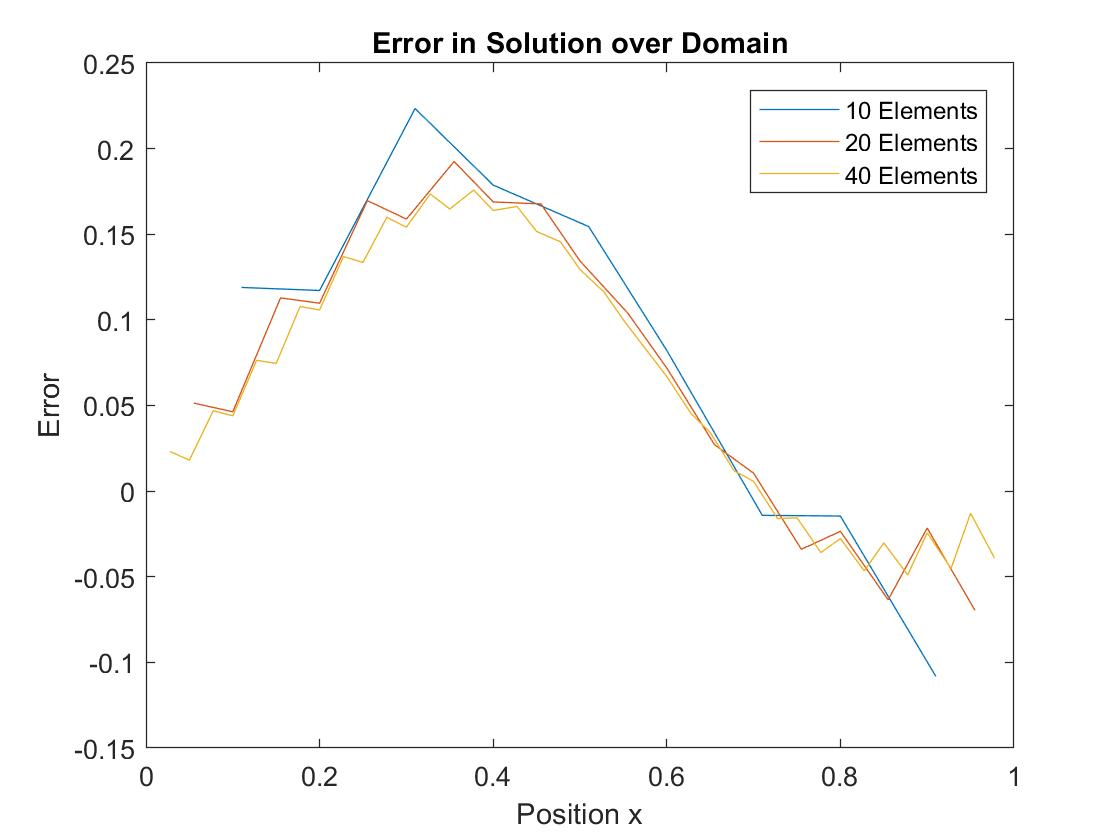
\includegraphics[width=11cm, height=11cm]{error}
  \caption{ Error in solution over domain of problem.}
  \label{fig:Error1}
\end{figure}

\begin{figure}[H]
  \centering
  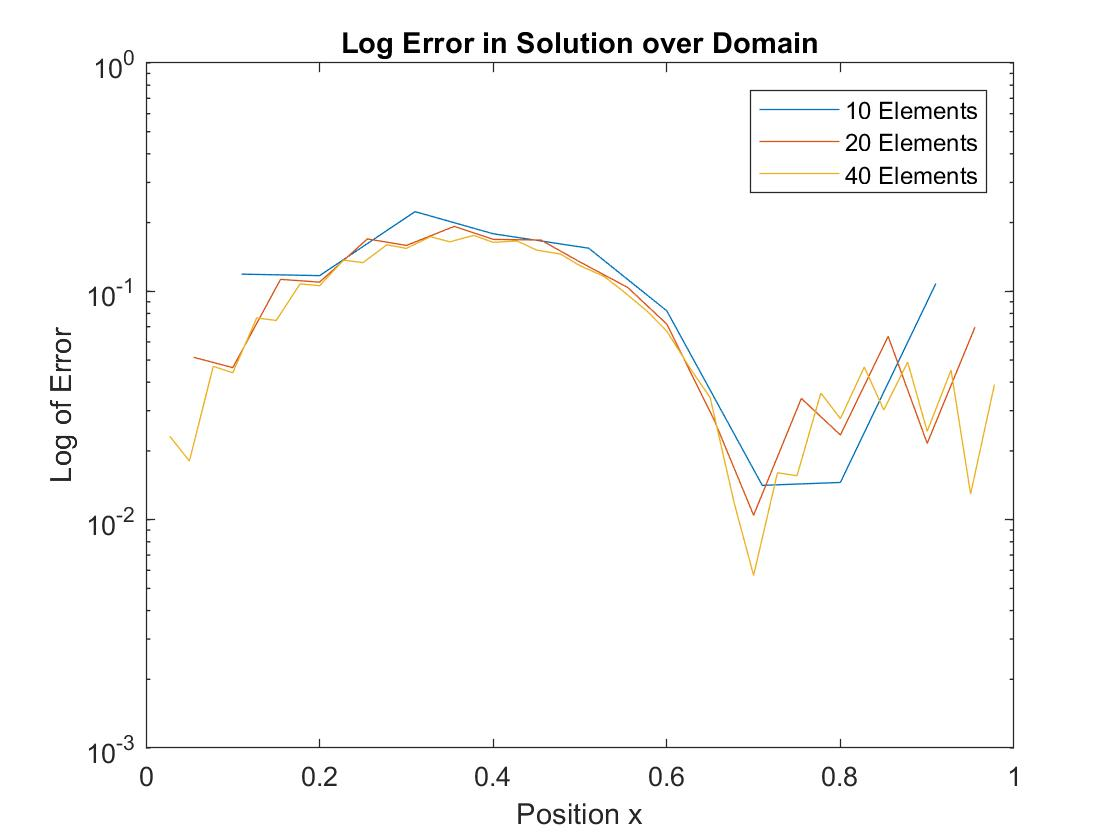
\includegraphics[width=11cm, height=11cm]{Log_error}
  \caption{ Log of error in solution over domain of problem.}
  \label{fig:Error2}
\end{figure}

\begin{table}[!ht]
\caption{Errors and convergence orders for Case 1.}
\vspace{0.1in}
\centering
\begin{tabular}{|c|c|c| c| c| c| c|}
\hline
 $N+1$&  $||e_h(\cdot)||_{L^2([0,1])}$ & Order  & $||e_h(\cdot)||_{L^\infty([0,1])}$ & Order& $||e_h(\cdot)||_h$& Order \\
 \hline
     10  &  2.072428e-02 & 0.00 & 2.233885e-01 & 0.00 & 1.884026e-01 & 0.00\\
     20  &  9.421318e-03 & 1.13 & 1.924613e-01 & 0.21 & 1.712967e-01 & 0.14\\
     40  &  3.740229e-03 & 1.33 & 1.758183e-01 & 0.13 & 1.360083e-01 & 0.33\\
     80  &  1.398561e-03 & 1.41 & 1.685136e-01 & 0.06 & 1.017135e-01 & 0.42\\
     160 &  5.082905e-04 & 1.46 & 1.646495e-01 & 0.03 & 7.393317e-02 & 0.46\\
     320 &  1.821839e-04 & 1.48 & 1.627100e-01 & 0.02 & 5.299896e-02 & 0.48\\
\hline
\end{tabular}
\label{tab:C1}
\end{table}

\begin{table}[!ht]
\caption{Errors and convergence orders for Case 2.}
\vspace{0.1in}
\centering
\begin{tabular}{|c|c|c| c| c| c| c|}
\hline
 $N+1$&  $||e_h(\cdot)||_{L^2([0,1])}$ & Order  & $||e_h(\cdot)||_{L^\infty([0,1])}$ & Order& $||e_h(\cdot)||_h$& Order \\
 \hline
     10  & 2.343497e-02 & 0.00 & 3.718547e-01  & 0.00 &  2.130452e-01 & 0.00 \\
     20  & 2.133812e-02 & 0.14 & 6.910094e-01  & -0.89 & 3.879659e-01 & -0.86\\
     40  & 1.097459e-02 & 0.96 & 9.852965e-01  & -0.51 & 3.990759e-01 & -4.07\\
     80  & 4.620878e-03 & 1.24 & 1.175112e+00  & -0.25 & 3.360638e-01 & 0.25\\
     160 & 1.780002e-03 & 1.37 & 1.278376e+00  & -0.12 & 2.589093e-01 & 0.37\\
     320 & 6.566801e-04 & 1.43 & 1.332562e+00  & -0.06 & 1.910342e-01 & 0.44\\
\hline
\end{tabular}
\label{tab:C2}
\end{table}

\begin{table}[!ht]
\caption{Errors and convergence orders for Case 3.}
\vspace{0.1in}
\centering
\begin{tabular}{|c|c|c| c| c| c| c|}
\hline
 $N+1$&  $||e_h(\cdot)||_{L^2([0,1])}$ & Order  & $||e_h(\cdot)||_{L^\infty([0,1])}$ & Order& $||e_h(\cdot)||_h$& Order \\
 \hline
     10  & 7.423628e-01 & 0.00 & 3.896897e+00 & 0.00  & 6.748753e+00 & 0.00 \\
     20  & 5.327322e-01 & 0.48 & 3.945805e+00 & -0.02 & 9.686040e+00 & -0.52\\
     40  & 3.797393e-01 & 0.49 & 3.972235e+00 & -0.01 & 1.380870e+01 & -0.51\\
     80  & 2.696418e-01 & 0.43 & 3.985950e+00 & -0.01 & 1.961031e+01 & -0.51\\
     160 & 1.910725e-01 & 0.49 & 3.992933e+00 & -0.01 & 2.779236e+01 & -0.50\\
     320 & 1.352541e-01 & 0.50 & 3.996456e+00 & -0.01 & 3.934665e+01 & -0.50\\
\hline
\end{tabular}
\label{tab:C3}
\end{table}

\begin{table}[!ht]
\caption{Errors and convergence orders for Case 4.}
\vspace{0.1in}
\centering
\begin{tabular}{|c|c|c| c| c| c| c|}
\hline
 $N+1$&  $||e_h(\cdot)||_{L^2([0,1])}$ & Order  & $||e_h(\cdot)||_{L^\infty([0,1])}$ & Order& $||e_h(\cdot)||_h$& Order \\
 \hline
     10  & 2.006381e-01 & 0.00  & 1.847478e+00 & 0.00  &1.823982e+00  & 0.00 \\
     20  & 1.385033e-01 & 0.53 &  1.922485e+00&  -0.05& 2.518242e+00 & -0.47\\
     40  & 9.681655e-02 & 0.52 &  1.960923e+00&  -0.02& 3.520602e+00 & -0.48\\
     80  & 6.807593e-02 & 0.51 &  1.980381e+00&  -0.01& 4.950977e+00 & -0.49\\
     160 & 4.800344e-02 & 0.50 &  1.990170e+00&  -0.01& 6.982319e+00 & -0.49\\
     320 & 3.389673e-02 & 0.50 &  1.995080e+00&  -0.01& 9.860868e+00 & -0.50\\
\hline
\end{tabular}
\label{tab:C4}
\end{table}

\begin{table}[!ht]
\caption{Errors and convergence orders for Case 5.}
\vspace{0.1in}
\centering
\begin{tabular}{|c|c|c| c| c| c| c|}
\hline
 $N+1$&  $||e_h(\cdot)||_{L^2([0,1])}$ & Order  & $||e_h(\cdot)||_{L^\infty([0,1])}$ & Order& $||e_h(\cdot)||_h$& Order \\
 \hline
     10  & 3.831430e-01 & 0.00 & 2.837704e+00 & 0.00  & 3.483118e+00 & 0.00\\
     20  & 2.704644e-01 & 0.50 & 2.917944e+00 & -0.04 & 4.917534e+00 & -0.49\\
     40  & 1.912960e-01 & 0.49 & 2.958735e+00 & -0.02 & 6.956220e+00 & -0.50\\
     80  & 1.353213e-01 & 0.49 & 2.979307e+00 & -0.09 & 9.841546e+00 & -0.50\\
     160 & 9.571245e-02 & 0.49 & 2.989638e+00 & -0.04 & 1.392181e+01 & -0.50\\
     320 & 6.768923e-02 & 0.49 & 2.994815e+00 & -0.02 & 1.969141e+01 & -0.50\\
\hline
\end{tabular}
\label{tab:C5}
\end{table}

\noindent
The following would was done to incorporate non-homogeneous Dirichlet boundary conditions.
First, the only change to the weak form of the problem would be separating the 
trial and test spaces; the solution must have a non-zero value on the specified 
boundary whereas the trial function must be zero on the boundaries.
For the FEM formulation, the contributions of the non-zero boundary
conditions are taken account for in the forcing vector. 
No changes need to be made to represent $U_h$ on \emph{interior} elements.
However, on the boundary, additional hat functions are used to recover the
assigned boundary values.
The matrix \textbf{A} is not changed as the original PDE does not change. 
The forcing vector \textbf{F} includes the addition of the boundary terms
on the first and last entry.


While the $L_2$ error norm decreases for all tests, the same is not true 
for the $L_\infty$ or the energy norm. Appended to the code is additional
work showing the hand calculations to derive the forcing functions and 
their approximated equivalents. The \texttt{Eigen} software package
was used as the linear solver for this project. 
The matrix inversion method used was Householder-QR with pivoting.

\newpage
\appendix
\section{Source Code and Headers} \label{sec:code}

\subsection{fea\_hw1.cpp} \label{subsec:fea_hw1.cpp}
\lstinputlisting{/lore/clougj/Learning_Codes/FEA/HW1/src/fea_hw1.cpp}

\subsection{driver.cpp} \label{subsec:driver.cpp}
\lstinputlisting{/lore/clougj/Learning_Codes/FEA/HW1/src/driver.cpp}
\subsection{driver.hpp} \label{subsec:driver.hpp}
\lstinputlisting{/lore/clougj/Learning_Codes/FEA/HW1/src/driver.hpp}

\subsection{element1D.cpp} \label{subsec:element1D.cpp}
\lstinputlisting{/lore/clougj/Learning_Codes/FEA/HW1/src/element1D.cpp}
\subsection{element1D.hpp} \label{subsec:element1D.hpp}
\lstinputlisting{/lore/clougj/Learning_Codes/FEA/HW1/src/element1D.hpp}

\subsection{errorCalcs.cpp} \label{subsec:errorCalcs.cpp}
\lstinputlisting{/lore/clougj/Learning_Codes/FEA/HW1/src/errorCalcs.cpp}
\subsection{errorCalcs.hpp} \label{subsec:errorCalcs.hpp}
\lstinputlisting{/lore/clougj/Learning_Codes/FEA/HW1/src/errorCalcs.hpp}

\subsection{forcing.cpp} \label{subsec:forcing.cpp}
\lstinputlisting{/lore/clougj/Learning_Codes/FEA/HW1/src/forcing.cpp}
\subsection{forcing.hpp} \label{subsec:forcing.hpp}
\lstinputlisting{/lore/clougj/Learning_Codes/FEA/HW1/src/forcing.hpp}

\subsection{mesh1D.cpp} \label{subsec:mesh1D.cpp}
\lstinputlisting{/lore/clougj/Learning_Codes/FEA/HW1/src/mesh1D.cpp}
\subsection{mesh1D.hpp} \label{subsec:mesh1D.hpp}
\lstinputlisting{/lore/clougj/Learning_Codes/FEA/HW1/src/mesh1D.hpp}

\subsection{stiffness.cpp} \label{subsec:stiffness.cpp}
\lstinputlisting{/lore/clougj/Learning_Codes/FEA/HW1/src/stiffness.cpp}
\subsection{stiffness.hpp} \label{subsec:stiffness.hpp}
\lstinputlisting{/lore/clougj/Learning_Codes/FEA/HW1/src/stiffness.hpp}

\subsection{eig\_wrap.hpp} \label{subsec:eig_wrap.hpp}
\lstinputlisting{/lore/clougj/Learning_Codes/FEA/HW1/src/eig_wrap.hpp}

\end{document}
